\documentclass[prl,reprint]{revtex4-1}
\usepackage{amsmath,amsfonts,amssymb}
\usepackage{graphicx}
\usepackage{braket}
\usepackage[bookmarks]{hyperref}
\begin{document}
\title{Path Integral Monte Carlo on Oscillators}
\author{Yubo Yang}

\newcommand{\tr}{\text{tr}}

\date{\today}
\begin{abstract}
Path integral Monte Carlo is implemented and applied to oscillators trapped by a central potential. 
\end{abstract}
\maketitle
\section{Context}
In the context of continuum-space path integral Monte Carlo (PIMC), the physical system to be studied is a collection of non-relativistic particles in three spatial dimensions each contributing a kinetic operator to the Hamiltonian $\hat{T}_j=\lambda_j(i\nabla_{\vec{r}_j})^2$, where $j=1,\cdots,N$ label the particles, and $\vec{r}_i$ is the position of particle $j$. Often $\lambda_j=\frac{1}{2m_j}$, where $m_j$ is the mass of the $j^{\text{th}}$ particle. Let the $3N$-vector $R=\{\vec{r}_j\}$ contain all $3N$ coordinates of the $N$ particles. Let the position basis that spans the Hilbert space of these particles be $\ket{R}$.

\section{Theory}
\subsection{The Density Matrix}
The thermal density matrix in operator notation is
\begin{align}
\hat{\rho} = e^{-\beta\hat{H}},
\end{align}
where $\hat{H}$ is the Hamiltonian and $\beta=\frac{1}{kT}$ is inverse temperature. It can be written in the position basis $\ket{R}$ and have the factorization property
\begin{align}
\rho(R_0,R_M;\beta)=\int[\prod_{t=1}^{M-1} dR_t]\prod_{t=1}^{M} \braket{R_{t-1}|e^{-\tau \hat{H}}|R_t}, \label{eq:factor}
\end{align}
where $M$ is an integer and $\tau=\beta/M$. If $\rho$ is to be viewed as a time evolution operator, then $\beta$ is the imaginary time of propagation. In this context, (\ref{eq:factor}) can be viewed as a discretization of the total propagation path of length $\beta$ into $M$ segments of length $\tau$. In the thermal dynamics context, the low temperature (quantum) behavior of the system is expressed as a convolution of high temperature (classical) behavior.
  
If $\tau$ is small enough and the Hamiltonian has separable kinetic and potential pieces $\hat{H}=\hat{T}+\hat{V}$, then each segment in (\ref{eq:factor}) can be separated using the Trotter formula
\begin{align}
\rho(R_{t-1},R_t;\tau)\equiv&\braket{R_{t-1}|e^{-\tau \hat{H}}|R_t}\approx\braket{R_{t-1}|e^{-\tau \hat{T}}e^{-\tau\hat{V}}|R_t}\nonumber \\
=&\int dR' \braket{R_{t-1}|e^{-\tau \hat{T}}|R'}\braket{R'|e^{-\tau\hat{V}}|R_t}, \label{eq:trotter}
\end{align}
which is exact in the limit $\tau\rightarrow0$~\cite{Bernu_book}. Assuming the potential is local, then $\braket{R'|e^{-\tau\hat{V}}|R_t}=e^{-\tau V(R_t)}\delta^{(3N)}(R'-R_t)$ and
\begin{align}
\rho(R_{t-1},R_t;\tau)=& \braket{R_{t-1}|e^{-\tau \hat{T}}|R_t}e^{-\tau V(R_t)}. \label{eq:local potential}
\end{align}
Recall each particle contributes a term $\hat{T}_j=\lambda_j(i\nabla_{\vec{r}_j})^2$ to the kinetic operator . To proceed, I will break up the particles into species, where all particles in a species have the same $\lambda$. Unless specified otherwise, I will only consider a single species in the rest of this document. Contributions from different species can be added together at the end. Assuming the particles are held in a 3D box with side length $L$, the kinetic piece can be evaluated by inserting a complete set of momentum states
\begin{align}
&\braket{R_{t-1}|e^{-\tau \hat{T}}|R_t}=\int dP\braket{R_{t-1}|P}\braket{P|e^{-\tau \hat{T}}|R_t} \nonumber \\
=&\sum_{n} L^{-3N}\exp\left\{-\tau\lambda 4\pi^2n\cdot n/L^2-2i\pi n\cdot(R_{t-1}-R_t)/L\right\} \nonumber \\
\approx& \frac{1}{(4\pi\lambda\tau)^{3N/2}}\exp\left(-\frac{(R_{t-1}-R_t)^2}{4\lambda\tau}\right). \label{eq:kinetic}
\end{align}
The last line is valid in the limit when the ``size'' of a particle is much smaller than the size of the box $\tau\lambda\ll L^2$, or when periodic boundary condition is used. Plugging (\ref{eq:trotter})-(\ref{eq:kinetic}) back into (\ref{eq:factor}) and we arrive at a practical expression for the thermal density matrix
\begin{align}
\rho(R_0,R_M;\beta)=&\int[\prod_{t=1}^{M-1} dR_t]\prod_{t=1}^{M} \frac{1}{(4\pi\lambda\tau)^{3N/2}}\times \nonumber \\
&\exp\left(-\tau(\frac{(R_{t-1}-R_t)^2}{4\lambda\tau^2}+V(R_t))\right) \nonumber \\
=&\frac{1}{(4\pi\lambda\tau)^{3MN/2}}\int[\prod_{t=1}^{M-1} dR_t] \nonumber \\
&\exp\left(-\tau\sum_{t=1}^M (\frac{(R_{t-1}-R_t)^2}{4\lambda\tau^2}+V(R_t)) \right) \nonumber \\
\propto& \int \mathcal{D}R~\exp (-\sum_{t=1}^M\tau L_{cl})~,
\end{align}
where $\int \mathcal{D}R\equiv \int[\prod_{t=1}^{M-1} dR_t]$ and the Classical Lagrangian~\cite{Ceperley_PIMC-review,Julich}
\begin{align}
L_{cl}(R_{t-1},R_t;\tau) \equiv \sum_{t=1}^M \frac{1}{4\lambda}\left(\frac{R_{t-1}-R_t}{\tau}\right)^2+V(R_t). \label{eq:Lcl}
\end{align}
The Classical Lagrangian is sufficient for later sampling, but for an exact expression for the density matrix, a constant term needs to be added in the \emph{primitive Lagrangian}
\begin{align}
&L^P_{cl}(R_{t-1},R_t;\tau)\equiv -\frac{1}{\tau}\ln\rho(R_{t-1},R_t;\tau) \nonumber \\
\approx&\frac{3N}{2\tau}\ln(4\pi\lambda\tau)+\frac{1}{4\lambda}\left(\frac{R_{t-1}-R_t}{\tau}\right)^2+V(R_t).
\end{align}
It is worth noting that the classical Lagrangian (\ref{eq:Lcl}) has a spring-like term and a potential term. This allows a classical interpretation of the quantum problem through an isomorphism with classical ring polymers.

\subsection{Classical Isomorphism}
To see a classical picture of the path integral formulation of the density matrix, we can break down the $3N$ vector $R$ into visualizable particle positions $r^{(i)}_j$.~\cite{Bernu_book} Now
\begin{align}
\sum_{t=1}^M (R_{t-1}-R_t)^2 =& \sum_{t=1}^M\sum_{j=1}^N (r^{(i)}_{t-1}-r^{(i)}_t)^2\nonumber \\
=&\sum_{j=1}^N\left(\sum_{t=1}^M (r^{(i)}_{t-1}-r^{(i)}_t)^2 \right).
\end{align}
That is, each particle can be visualized as a collection of beads, one at each imaginary time slice. In this context, the kinetic contribution (\ref{eq:kinetic}) to the classical action can be considered particle-by-particle
\begin{align}
\left(\sum_{t=1}^M\frac{(R_{t-1}-R_t)^2}{4\lambda\tau}\right)_i=\sum_{t=1}^M \frac{(r^{(i)}_{t-1}-r^{(i)}_t)^2}{4\lambda\tau}.
\end{align}
This term can be interpreted as series of a spring potentials coupling beads belonging to the same particle $i$ at adjacent time slices.

\subsection{The Partition Function and Observables}
The partition function can be evaluated as a trace of the density matrix
\begin{align}
Z(\beta)=& \int dR~\rho(R,R;\beta) \nonumber \\
=&\lim_{M\rightarrow\infty} \int \mathcal{D}R~\exp\left(-\sum_{t=1}^M\tau L_{cl}^P(R_{t-1},R_t;\tau)\right) \nonumber \\
\equiv& \int \mathcal{D}R~\exp\left(-S_{cl}^P(R,R;\beta)\right),
\end{align}
which is of path integral form. The expectation value of any operator $\mathcal{\hat{O}}$ can be formally written as an operator insertion in the path integral
\begin{align}
\braket{\mathcal{\hat{O}}}=\tr(\hat{O}\hat{\rho})=\int \mathcal{D}R~\hat{\mathcal{O}}\exp\left(-S_{cl}^P\right).
\end{align}
Due to the cyclic nature of trace, $\hat{O}$ can be inserted between any two segments (time slices) in a discretized path integral. If the operator is local in space, then $\hat{\mathcal{O}}_l$ can be evaluated at a single time slice
\begin{align}
\braket{\mathcal{\hat{O}}_l}=\frac{1}{Z}\int \mathcal{D}R~\mathcal{O}_l(R_t)\exp\left(-S_{cl}^P\right),
\end{align}
for any $t=1,\dots,M$. Although in practice, one may choose to average over all $M$ time slices to obtain better statistics
\begin{align}
\braket{\mathcal{\hat{O}}_l} \leftarrow \frac{1}{N}\sum_{t=1}^M \mathcal{O}_l(R_{t}) \label{eq:Ol}
\end{align}
 The expectation value of the kinetic operator can be evaluated by a derivative against imaginary time. Notice
\begin{align}
&\braket{R_{t-1}|\hat{T}e^{-\tau\hat{T}}|R_t}=-\frac{\partial}{\partial\tau}\braket{R_{t-1}|e^{-\tau\hat{T}}|R_t}\nonumber \\
\approx&-\frac{\partial}{\partial\tau}\frac{1}{(4\pi\lambda\tau)^{3N/2}}\exp\left(-\frac{(R_{t-1}-R_t)^2}{4\lambda\tau}\right) \nonumber \\
=&\left(\frac{3N}{2\tau}-\frac{1}{4\lambda}(\frac{R_{t-1}-R_t}{\tau})^2\right)\frac{\exp\left(-\frac{(R_{t-1}-R_t)^2}{4\lambda\tau}\right)}{(4\pi\lambda\tau)^{3N/2}} \nonumber \\
\approx& \left(\frac{3N}{2\tau}-\frac{1}{4\lambda}(\frac{R_{t-1}-R_t}{\tau})^2\right)\braket{R_{t-1}|e^{-\tau\hat{T}}|R_t}.
\end{align}
Therefore the kinetic energy evaluation involves two adjacent time slices. Again, for better statistics
\begin{align}
\braket{\hat{T}} \leftarrow \frac{3N}{2\tau}-\frac{1}{4\lambda\tau^2}\frac{1}{M}\sum_{t=1}^M(R_{t-1}-R_t)^2. \label{eq:T}
\end{align}

Now we can simulate the classical system of $M\times N$ particles according to the classical action (\ref{eq:Lcl}), record observables according to formulae such as (\ref{eq:Ol}) and (\ref{eq:T}) to solve the quantum system of $N$ particles.

\section{Implementation}

The classical isomorphism makes the implementation of PIMC fairly straight forward. In particular, I will use the Metropolis algorithm to sample classical ring polymer configurations according to the classical action. Each configuration is defined by a 3-dimensional array Rti of size ($M$,$N$,$3$), which contains the spatial locations of the $M\times N$ classical beads or equivalently, a \emph{path}.

From an initial path, $p_1$, some move will be proposed with probability $T(p_1\rightarrow p_2)$ and accepted with the Metropolis acceptance rate 
\begin{align}
A = \text{min}\left\{\frac{\exp(-S_{cl}(p_2))}{\exp(-S_{cl}(p2))}\frac{T(p_2\rightarrow p_1)}{T(p_1\rightarrow p_2)}\right\},
\end{align}
and observables will be accumulated. Different forms of the transfer matrix $T(p_1\rightarrow p_2)$ can be explored for an efficient sampling algorithm.

\subsection{A Single Oscillator Trapped by a Central Potential}
For the simplest case, I will consider a single harmonic oscillator of mass $m$ trapped by a harmonic potential~\cite{QMC_book}
\begin{align}
V(\vec{r}) = \frac{1}{2}m\omega^2r^2,
\end{align}
where $\vec{r}$ is the position of the oscillator. The Hamiltonian
\begin{align}
H=\lambda (i\vec{\nabla})^2+\frac{1}{2}m\omega^2r^2,
\end{align}
in three spatial dimensions has eigenvalues
\begin{align}
E(n_x,n_y,n_z) = \hbar\omega(n_x+n_y+n_z+\frac{3}{2}).
\end{align}
The partition function
\begin{align}
Z =& \sum_{n_x=0}^\infty\sum_{n_y=0}^\infty\sum_{n_z=0}^\infty \exp\left(-\beta E(n_x,n_y,n_z)\right) \nonumber \\
=&\frac{1}{8}\text{csch}^3(\frac{1}{2}\beta\hbar\omega).
\end{align}
The expectation energy can then be calculated as
\begin{align}
\braket{E} = -\partial_\beta\ln Z=\frac{3}{2}\hbar\omega\coth(\frac{1}{2}\beta\hbar\omega).
\end{align}

\begin{figure}[h]
\centering
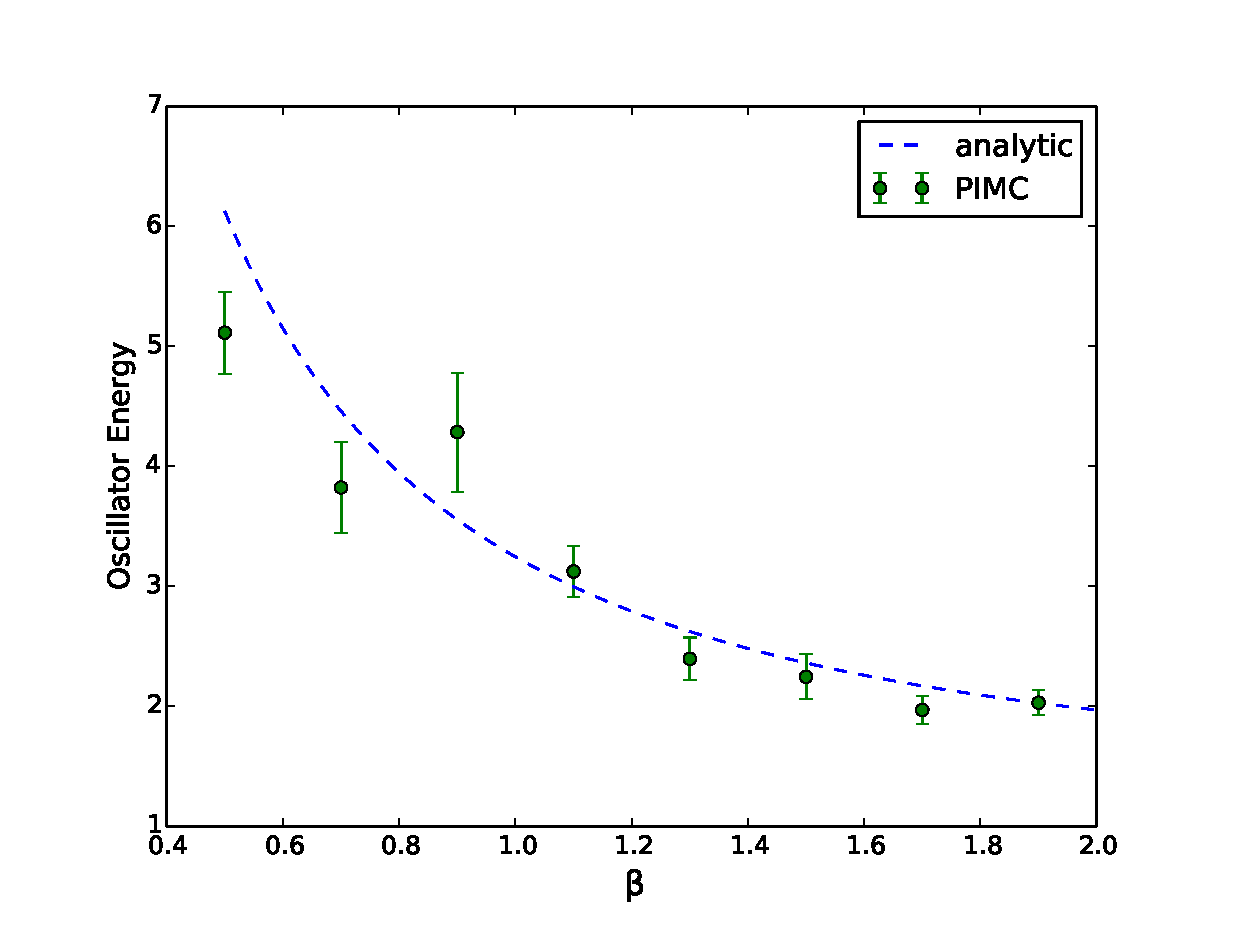
\includegraphics[scale=.4]{figures/single-harmonic}
\caption{Energy of a single harmonic oscillator calculated with PIMC and analytically.\label{fig:single-harmonic}}
\end{figure}

PIMC simulation was performed for a single harmonic oscillator with unit mass and unit frequency in atomic units $m=\omega=\hbar=1$. The PIMC results matches the analytical solution as shown in Figure \ref{fig:single-harmonic}. Single bead moves are used, but displacement moves and bisection moves can be implemented and integrated with the main code in a straight forward manner. Pair potential can be added as a subtype of the potential type. Please see details of the implementation in the jupyter notebook inside my GitHub folder ``algorithmic-perspective/PIMC/pimc.ipynb". 

\section{Appendix}
The kinetic integral can be performed by completing the square
%\begin{widetext}
\begin{align*}
\int dp~e^{ip\cdot(R_{t-1}-R_t)+\lambda\tau p} =& \frac{1}{(4\pi\lambda\tau)^{3N/2}}\times \\
&\exp\left\{-\frac{(R_{t-1}-R_t)^2}{4\lambda\tau}\right\}
\end{align*}
%\end{widetext}

\bibliographystyle{unsrt}
\bibliography{ref}



\end{document}